% !TeX spellcheck = ru_RU
% !TEX root=../main.tex

\begin{lecture}[Растворы и взаимная растворяемость]
	Вследствие шубы имеем поправку на потенциал: $ \phi (r) = \dfrac{e^2}{\eps r} e^{-\kappa r} $.
	Характерный радиус $ \lambda  = \sqrt{\dfrac{\eps k T}{8 \pi e^2 n}}~\Rightarrow~ U = -\dfrac{e^2 \kappa}{\eps}$.
	\begin{lecSection}[Ионные жидкости]
		При $ T \rightarrow 800^\circ C $ расплав, $ 10 - 25 \% $, % TODO: ЧТО ТАМ НАПИСАНО В КОНСПЕКТЕ??
		
		То есть, \underline{в структуре расплава появляются полости}.
		
		Есть вещества, являющиеся ионными жидкостями при комнатной температуре, например, RTIL.
		\begin{figure}[h]
			\centering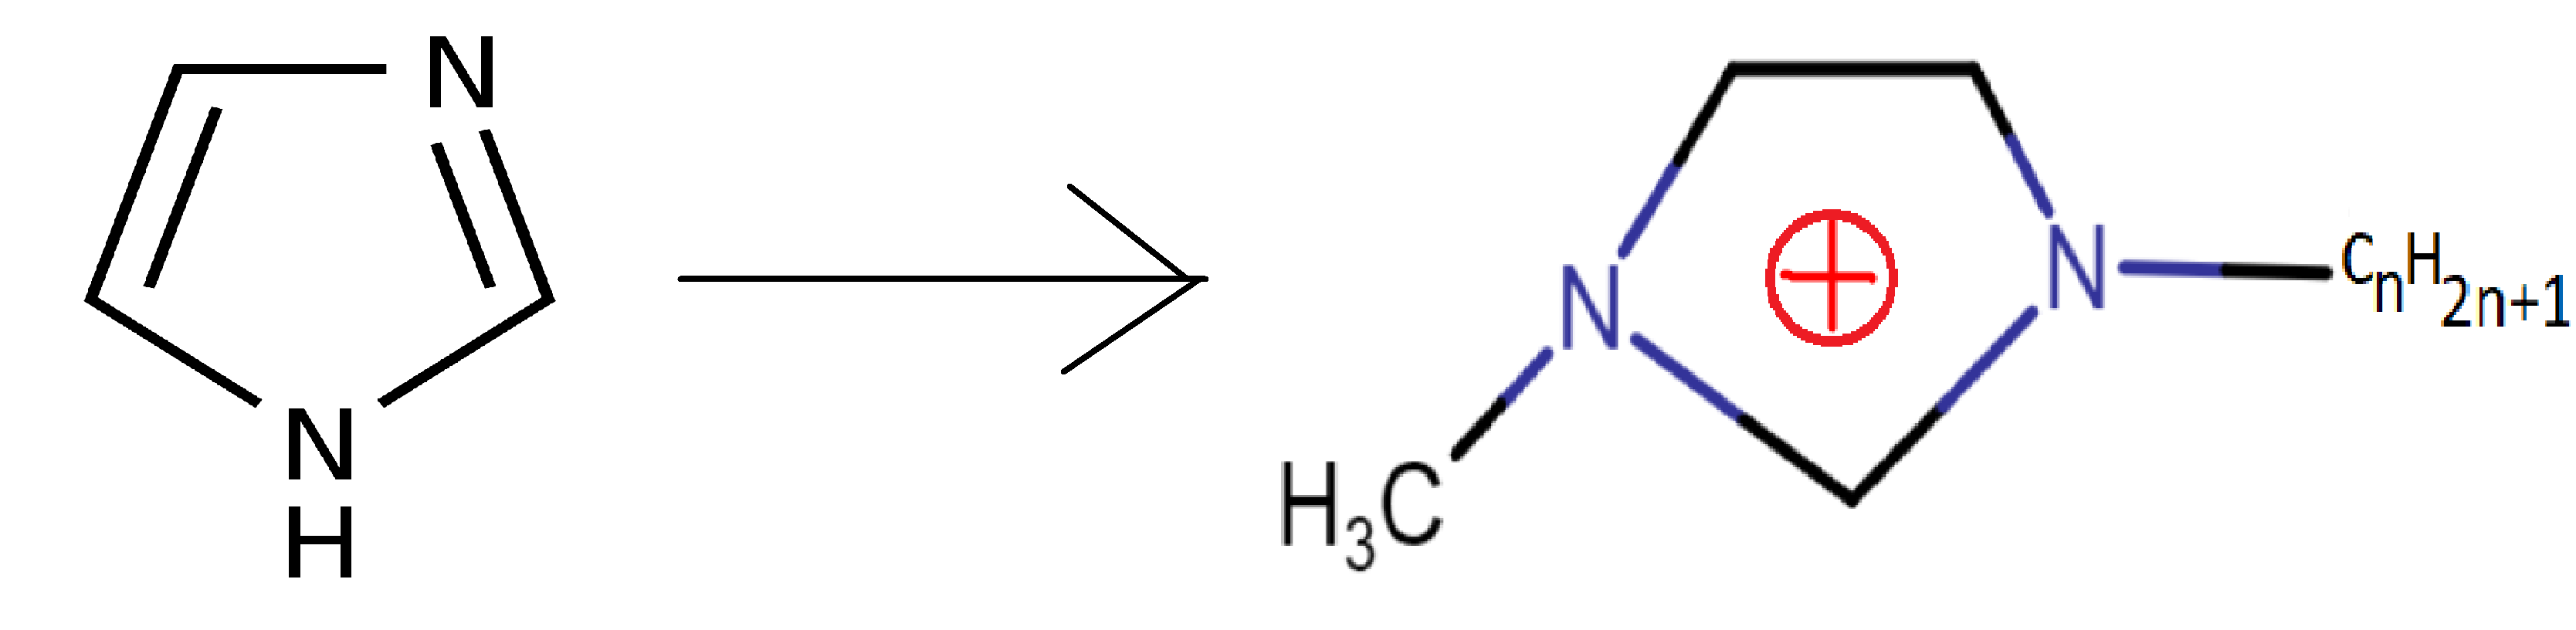
\includegraphics[width=0.8\linewidth]{lecture_11/imidazole}
			\caption{Превращение имидазола}
			\label{fig:11:imid_transform}
		\end{figure}
		
		\begin{figure}[h]
			\begin{minipage}{0.48\linewidth}
				\centering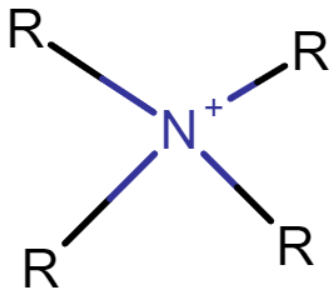
\includegraphics[width=0.7\linewidth]{lecture_11/alkil_ammon}
				\caption{Алкиламмоний}
				\label{fig:11:alkilammon}
			\end{minipage}
			\begin{minipage}{0.48\linewidth}
				\centering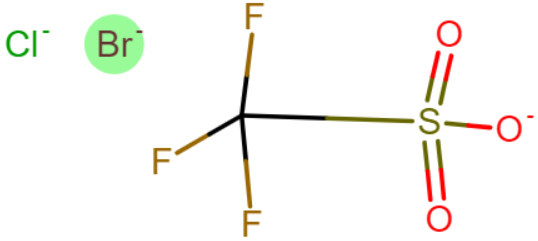
\includegraphics[width=\linewidth]{lecture_11/pic3}
				\caption{3-флюрометан сульфонат}
				\label{fig:11:metan_sulfonat}
			\end{minipage}
		\end{figure}
	
		ИЖ -- нелетучие, негорючие, наноразмерные неоднородности, $ \eps \sim 10 $, высокая вязкость.
		
		Можно смешивать с органическими растворами, что снижает вязкость.
		
		\underline{Использование}:
		\begin{itemize}
			\item Медицина (комплекс)
			\item В качестве растворителей
			\item В ядерных технология (жидкая экстракция)
		\end{itemize}
	
		\textit{Пример}: несмешиваемые $ A $ и $ B $. При этом $ C $ растворяется в обоих. Как распределится $ C $ между $ A $ и $ B $?
		
		\begin{gather*}
			d G = \sum\limits_i \mu_i dN_i = 0 ~\text{-- общая формула} \\
			= \mu_A dn_A - \mu_B dn_A = 0
		\end{gather*}
		где $ \mu_A $ -- потенциал в $ A $, $ \mu_A = \mu_B $ в равновесии.
		\begin{gather*}
		\mu_A^0 + RT \ln C_A = \mu_B^0 + RT \ln C_B \\
		\dfrac{C_A}{C_B} = \exp \left( \dfrac{\mu_B^0 - \mu_A^0}{RT}\right) = D~\text{-- коэффициент распределения}
		\end{gather*}
		
		\textit{Пример 2}: растворение $ I_2 $ в воде и в $ CCl_4 $ (которые не перемешиваются между собой).
		
		\begin{equation*}
		I_2 (\text{водн.}) \rightleftharpoons I_2 (CCl_4)
		\label{chem:iod_in_two_solvators}
		\end{equation*}
		
		Мы знаем, что $ D = 100 $.
		Пусть изначально было $ I_2^0 $.
		
		\begin{gather*}
		N_{I_2} = V_\text{в} I_2^0 \\
		\Rightarrow V_\text{в} C_2^0 = V_\text{в} C_\text{в}^1 + V_0 C_C^1, ~~ C_\text{в}^1 = \dfrac{1}{1 + D \cfrac{V_0}{V_\text{в}}}\, C_\text{в}^0
		\end{gather*}
		
		Пусть $ V_\text{в} = 100, ~ V_0 = 10, ~ \Rightarrow C_\text{в}^1 = \dfrac{C_\text{в}^0}{11} $.
	\end{lecSection}
	\begin{lecSection}[Метод корреляционных функций для описания систем]
		$ N = \text{const}; ~~ T, V = \text{const} $; в квантовой системе $ \eps \in \{\eps_i\} $
		\begin{gather*}
			Z = \sum\limits_i e^{-\beta \eps_i}, ~ \beta = \cfrac{1}{kT} \\
			A (T, V, N) = - kT \ln Z(T, V, N) ~ \text{-- статистическйи мостик} \\
			p = - \left( \dfrac{\partial A}{\partial V} \right)_{T, N}
		\end{gather*}
		
		Есть другой подход:
		
		\begin{center}\begin{tabular}{ll}
			& $ dV_1, dV_2, \dots, dV_n, ~ n \leq N $ -- где находится частица \\
			& $ d\phi (\vec{r_1}, \dots, \vec{r_n}) = F_n (\vec{r_1}, \vec{r_2}, \dots, \vec{r_n}) \dfrac{dV_1 dV_2 \dots dV_n}{V^n} $ \\
			\multicolumn{2}{c}{Вся информация известна, если известны все $ F_n, V_n $}
		\end{tabular}\end{center}
	
		Вводится нормировка: $ \int \dots \int F_n \dfrac{d^n V}{V^n} = 1 $, $ dV_1 = 4\pi R_i^2 dR_i $.
		
		Корреляция --- степень зависимости двух процессов в разных точках пространства.
		
		\begin{gather*}
			d p_1 = F_1 (R_1) \,\dfrac{V_1}{V} ~ \text{-- плотность частиц} \\
			d p_2 = F_2 (R_1 R_2) \,\dfrac{dV_1 dV_2}{V^2} ~ \text{-- бинарная функция распределения}
		\end{gather*}
	\end{lecSection}
\end{lecture}